%%%%%%%%%%%%%%%%%%%%%%%%%%%%%%%%%%%%%%%%%
% The Legrand Orange Book
% LaTeX Template
% Version 2.4 (26/09/2018)
%
% This template was downloaded from:
% http://www.LaTeXTemplates.com
%
% Original author:
% Mathias Legrand (legrand.mathias@gmail.com) with modifications by:
% Vel (vel@latextemplates.com)
%
% License:
% CC BY-NC-SA 3.0 (http://creativecommons.org/licenses/by-nc-sa/3.0/)
%
% Compiling this template:
% This template uses biber for its bibliography and makeindex for its index.
% When you first open the template, compile it from the command line with the 
% commands below to make sure your LaTeX distribution is configured correctly:
%
% 1) pdflatex main
% 2) makeindex main.idx -s StyleInd.ist
% 3) biber main
% 4) pdflatex main x 2
%
% After this, when you wish to update the bibliography/index use the appropriate
% command above and make sure to compile with pdflatex several times 
% afterwards to propagate your changes to the document.
%
% This template also uses a number of packages which may need to be
% updated to the newest versions for the template to compile. It is strongly
% recommended you update your LaTeX distribution if you have any
% compilation errors.
%
% Important note:
% Chapter heading images should have a 2:1 width:height ratio,
% e.g. 920px width and 460px height.
%
%%%%%%%%%%%%%%%%%%%%%%%%%%%%%%%%%%%%%%%%%

%----------------------------------------------------------------------------------------
%	PACKAGES AND OTHER DOCUMENT CONFIGURATIONS
%----------------------------------------------------------------------------------------

\documentclass[12pt,fleqn]{book} % Default font size and left-justified equations

%%%%%%%%%%%%%%%%%%%%%%%%%%%%%%%%%%%%%%%%%
% The Legrand Orange Book
% Structural Definitions File
% Version 2.1 (26/09/2018)
%
% Original author:
% Mathias Legrand (legrand.mathias@gmail.com) with modifications by:
% Vel (vel@latextemplates.com)
% 
% This file was downloaded from:
% http://www.LaTeXTemplates.com
%
% License:
% CC BY-NC-SA 3.0 (http://creativecommons.org/licenses/by-nc-sa/3.0/)
%
%%%%%%%%%%%%%%%%%%%%%%%%%%%%%%%%%%%%%%%%%

%----------------------------------------------------------------------------------------
%	VARIOUS REQUIRED PACKAGES AND CONFIGURATIONS
%----------------------------------------------------------------------------------------

\usepackage{graphicx} % Required for including pictures
\graphicspath{{Pictures/}} % Specifies the directory where pictures are stored

\usepackage{lipsum} % Inserts dummy text

\usepackage{tikz} % Required for drawing custom shapes

\usepackage[english]{babel} % English language/hyphenation

\usepackage{enumitem} % Customize lists
\setlist{nolistsep} % Reduce spacing between bullet points and numbered lists

\usepackage{booktabs} % Required for nicer horizontal rules in tables

\usepackage{xcolor} % Required for specifying colors by name
\definecolor{ocre}{RGB}{243,102,25} % Define the orange color used for highlighting throughout the book


%----------------------------------------------------------------------------------------
%	MARGINS
%----------------------------------------------------------------------------------------

\usepackage{geometry} % Required for adjusting page dimensions and margins

\geometry{
	paper=a4paper, % Paper size, change to letterpaper for US letter size
	top=3cm, % Top margin
	bottom=3cm, % Bottom margin
	left=3cm, % Left margin
	right=3cm, % Right margin
	headheight=14pt, % Header height
	footskip=1.4cm, % Space from the bottom margin to the baseline of the footer
	headsep=10pt, % Space from the top margin to the baseline of the header
	%showframe, % Uncomment to show how the type block is set on the page
}

%----------------------------------------------------------------------------------------
%	FONTS
%----------------------------------------------------------------------------------------

\usepackage{avant} % Use the Avantgarde font for headings
%\usepackage{times} % Use the Times font for headings
\usepackage{mathptmx} % Use the Adobe Times Roman as the default text font together with math symbols from the Sym­bol, Chancery and Com­puter Modern fonts

\usepackage{microtype} % Slightly tweak font spacing for aesthetics
\usepackage[utf8]{inputenc} % Required for including letters with accents
\usepackage[T1]{fontenc} % Use 8-bit encoding that has 256 glyphs

%----------------------------------------------------------------------------------------
%	BIBLIOGRAPHY AND INDEX
%----------------------------------------------------------------------------------------

\usepackage[style=numeric,citestyle=numeric,sorting=nyt,sortcites=true,autopunct=true,babel=hyphen,hyperref=true,abbreviate=false,backref=true,backend=biber]{biblatex}
\addbibresource{bibliography.bib} % BibTeX bibliography file
\defbibheading{bibempty}{}

\usepackage{calc} % For simpler calculation - used for spacing the index letter headings correctly
\usepackage{makeidx} % Required to make an index
\makeindex % Tells LaTeX to create the files required for indexing

%----------------------------------------------------------------------------------------
%	MAIN TABLE OF CONTENTS
%----------------------------------------------------------------------------------------

\usepackage{titletoc} % Required for manipulating the table of contents

\contentsmargin{0cm} % Removes the default margin

% Part text styling (this is mostly taken care of in the PART HEADINGS section of this file)
\titlecontents{part}
	[0cm] % Left indentation
	{\addvspace{20pt}\bfseries} % Spacing and font options for parts
	{}
	{}
	{}

% Chapter text styling
\titlecontents{chapter}
	[1.25cm] % Left indentation
	{\addvspace{12pt}\large\sffamily\bfseries} % Spacing and font options for chapters
	{\color{ocre!60}\contentslabel[\Large\thecontentslabel]{1.25cm}\color{ocre}} % Formatting of numbered sections of this type
	{\color{ocre}} % Formatting of numberless sections of this type
	{\color{ocre!60}\normalsize\;\titlerule*[.5pc]{.}\;\thecontentspage} % Formatting of the filler to the right of the heading and the page number

% Section text styling
\titlecontents{section}
	[1.25cm] % Left indentation
	{\addvspace{3pt}\sffamily\bfseries} % Spacing and font options for sections
	{\contentslabel[\thecontentslabel]{1.25cm}} % Formatting of numbered sections of this type
	{} % Formatting of numberless sections of this type
	{\hfill\color{black}\thecontentspage} % Formatting of the filler to the right of the heading and the page number

% Subsection text styling
\titlecontents{subsection}
	[1.25cm] % Left indentation
	{\addvspace{1pt}\sffamily\small} % Spacing and font options for subsections
	{\contentslabel[\thecontentslabel]{1.25cm}} % Formatting of numbered sections of this type
	{} % Formatting of numberless sections of this type
	{\ \titlerule*[.5pc]{.}\;\thecontentspage} % Formatting of the filler to the right of the heading and the page number

% Figure text styling
\titlecontents{figure}
	[1.25cm] % Left indentation
	{\addvspace{1pt}\sffamily\small} % Spacing and font options for figures
	{\thecontentslabel\hspace*{1em}} % Formatting of numbered sections of this type
	{} % Formatting of numberless sections of this type
	{\ \titlerule*[.5pc]{.}\;\thecontentspage} % Formatting of the filler to the right of the heading and the page number

% Table text styling
\titlecontents{table}
	[1.25cm] % Left indentation
	{\addvspace{1pt}\sffamily\small} % Spacing and font options for tables
	{\thecontentslabel\hspace*{1em}} % Formatting of numbered sections of this type
	{} % Formatting of numberless sections of this type
	{\ \titlerule*[.5pc]{.}\;\thecontentspage} % Formatting of the filler to the right of the heading and the page number

%----------------------------------------------------------------------------------------
%	MINI TABLE OF CONTENTS IN PART HEADS
%----------------------------------------------------------------------------------------

% Chapter text styling
\titlecontents{lchapter}
	[0em] % Left indentation
	{\addvspace{15pt}\large\sffamily\bfseries} % Spacing and font options for chapters
	{\color{ocre}\contentslabel[\Large\thecontentslabel]{1.25cm}\color{ocre}} % Chapter number
	{}  
	{\color{ocre}\normalsize\sffamily\bfseries\;\titlerule*[.5pc]{.}\;\thecontentspage} % Page number

% Section text styling
\titlecontents{lsection}
	[0em] % Left indentation
	{\sffamily\small} % Spacing and font options for sections
	{\contentslabel[\thecontentslabel]{1.25cm}} % Section number
	{}
	{}

% Subsection text styling (note these aren't shown by default, display them by searchings this file for tocdepth and reading the commented text)
\titlecontents{lsubsection}
	[.5em] % Left indentation
	{\sffamily\footnotesize} % Spacing and font options for subsections
	{\contentslabel[\thecontentslabel]{1.25cm}}
	{}
	{}

%----------------------------------------------------------------------------------------
%	HEADERS AND FOOTERS
%----------------------------------------------------------------------------------------

\usepackage{fancyhdr} % Required for header and footer configuration

\pagestyle{fancy} % Enable the custom headers and footers

\renewcommand{\chaptermark}[1]{\markboth{\sffamily\normalsize\bfseries\chaptername\ \thechapter.\ #1}{}} % Styling for the current chapter in the header
\renewcommand{\sectionmark}[1]{\markright{\sffamily\normalsize\thesection\hspace{5pt}#1}{}} % Styling for the current section in the header

\fancyhf{} % Clear default headers and footers
\fancyhead[LE,RO]{\sffamily\normalsize\thepage} % Styling for the page number in the header
\fancyhead[LO]{\rightmark} % Print the nearest section name on the left side of odd pages
\fancyhead[RE]{\leftmark} % Print the current chapter name on the right side of even pages
%\fancyfoot[C]{\thepage} % Uncomment to include a footer

\renewcommand{\headrulewidth}{0.5pt} % Thickness of the rule under the header

\fancypagestyle{plain}{% Style for when a plain pagestyle is specified
	\fancyhead{}\renewcommand{\headrulewidth}{0pt}%
}

% Removes the header from odd empty pages at the end of chapters
\makeatletter
\renewcommand{\cleardoublepage}{
\clearpage\ifodd\c@page\else
\hbox{}
\vspace*{\fill}
\thispagestyle{empty}
\newpage
\fi}

%----------------------------------------------------------------------------------------
%	THEOREM STYLES
%----------------------------------------------------------------------------------------

\usepackage{tikz}
\newcommand\pacman[2]{\tikz[baseline, #1]{%
    \draw[thick,fill=#2]
    (0,0) -- (30:1cm) arc (30:330:1cm) -- cycle;
    \fill (0,2/3) circle (1.5mm);}
                       } 
                      

\usepackage{amsmath,amsfonts,amssymb,amsthm} % For math equations, theorems, symbols, etc

\newcommand{\intoo}[2]{\mathopen{]}#1\,;#2\mathclose{[}}
\newcommand{\ud}{\mathop{\mathrm{{}d}}\mathopen{}}
\newcommand{\intff}[2]{\mathopen{[}#1\,;#2\mathclose{]}}
\renewcommand{\qedsymbol}{$\blacksquare$}
\newtheorem{notation}{Notation}[chapter]

% Boxed/framed environments
\newtheoremstyle{ocrenumbox}% Theorem style name
{0pt}% Space above
{0pt}% Space below
{\normalfont}% Body font
{}% Indent amount
{\small\bf\sffamily\color{ocre}}% Theorem head font
{\;}% Punctuation after theorem head
{0.25em}% Space after theorem head
{\small\sffamily\color{ocre}\thmname{#1}\nobreakspace\thmnumber{\@ifnotempty{#1}{}\@upn{#2}}% Theorem text (e.g. Theorem 2.1)
\thmnote{\nobreakspace\the\thm@notefont\sffamily\bfseries\color{black}---\nobreakspace#3.}} % Optional theorem note

\newtheoremstyle{blacknumex}% Theorem style name
{5pt}% Space above
{5pt}% Space below
{\normalfont}% Body font
{} % Indent amount
{\small\bf\sffamily}% Theorem head font
{\;}% Punctuation after theorem head
{0.25em}% Space after theorem head
{\small\sffamily{\tiny\ensuremath{\blacksquare}}\nobreakspace\thmname{#1}\nobreakspace\thmnumber{\@ifnotempty{#1}{}\@upn{#2}}% Theorem text (e.g. Theorem 2.1)
\thmnote{\nobreakspace\the\thm@notefont\sffamily\bfseries---\nobreakspace#3.}}% Optional theorem note

\newtheoremstyle{blacknumbox} % Theorem style name
{0pt}% Space above
{0pt}% Space below
{\normalfont}% Body font
{}% Indent amount
{\small\bf\sffamily}% Theorem head font
{\;}% Punctuation after theorem head
{0.25em}% Space after theorem head
{\small\sffamily\thmname{#1}\nobreakspace\thmnumber{\@ifnotempty{#1}{}\@upn{#2}}% Theorem text (e.g. Theorem 2.1)
\thmnote{\nobreakspace\the\thm@notefont\sffamily\bfseries---\nobreakspace#3.}}% Optional theorem note

% Non-boxed/non-framed environments
\newtheoremstyle{ocrenum}% Theorem style name
{5pt}% Space above
{5pt}% Space below
{\normalfont}% Body font
{}% Indent amount
{\small\bf\sffamily\color{ocre}}% Theorem head font
{\;}% Punctuation after theorem head
{0.25em}% Space after theorem head
{\small\sffamily\color{ocre}\thmname{#1}\nobreakspace\thmnumber{\@ifnotempty{#1}{}\@upn{#2}}% Theorem text (e.g. Theorem 2.1)
\thmnote{\nobreakspace\the\thm@notefont\sffamily\bfseries\color{black}---\nobreakspace#3.}} % Optional theorem note
\makeatother

% Defines the theorem text style for each type of theorem to one of the three styles above
\newcounter{dummy} 
\numberwithin{dummy}{section}
\theoremstyle{ocrenumbox}
\newtheorem{theoremeT}[dummy]{Theorem}
\newtheorem{problem}{Problem}[chapter]
\newtheorem{exerciseT}{Exercise}[chapter]
\theoremstyle{blacknumex}
\newtheorem{exampleT}{Example}[chapter]
\theoremstyle{blacknumbox}
\newtheorem{vocabulary}{Vocabulary}[chapter]
\newtheorem{definitionT}{Definition}[section]
\newtheorem{corollaryT}[dummy]{Corollary}
\theoremstyle{ocrenum}
\newtheorem{proposition}[dummy]{Proposition}

%----------------------------------------------------------------------------------------
%	DEFINITION OF COLORED BOXES
%----------------------------------------------------------------------------------------

\RequirePackage[framemethod=default]{mdframed} % Required for creating the theorem, definition, exercise and corollary boxes

% Theorem box
\newmdenv[skipabove=7pt,
skipbelow=7pt,
backgroundcolor=black!5,
linecolor=ocre,
innerleftmargin=5pt,
innerrightmargin=5pt,
innertopmargin=5pt,
leftmargin=0cm,
rightmargin=0cm,
innerbottommargin=5pt]{tBox}

% Exercise box	  
\newmdenv[skipabove=7pt,
skipbelow=7pt,
rightline=false,
leftline=true,
topline=false,
bottomline=false,
backgroundcolor=ocre!10,
linecolor=ocre,
innerleftmargin=5pt,
innerrightmargin=5pt,
innertopmargin=5pt,
innerbottommargin=5pt,
leftmargin=0cm,
rightmargin=0cm,
linewidth=4pt]{eBox}	

% Definition box
\newmdenv[skipabove=7pt,
skipbelow=7pt,
rightline=false,
leftline=true,
topline=false,
bottomline=false,
linecolor=ocre,
innerleftmargin=5pt,
innerrightmargin=5pt,
innertopmargin=0pt,
leftmargin=0cm,
rightmargin=0cm,
linewidth=4pt,
innerbottommargin=0pt]{dBox}	

% Corollary box
\newmdenv[skipabove=7pt,
skipbelow=7pt,
rightline=false,
leftline=true,
topline=false,
bottomline=false,
linecolor=gray,
backgroundcolor=black!5,
innerleftmargin=5pt,
innerrightmargin=5pt,
innertopmargin=5pt,
leftmargin=0cm,
rightmargin=0cm,
linewidth=4pt,
innerbottommargin=5pt]{cBox}

% Creates an environment for each type of theorem and assigns it a theorem text style from the "Theorem Styles" section above and a colored box from above
\newenvironment{theorem}{\begin{tBox}\begin{theoremeT}}{\end{theoremeT}\end{tBox}}
\newenvironment{exercise}{\begin{eBox}\begin{exerciseT}}{\hfill{\color{ocre}\tiny\ensuremath{\blacksquare}}\end{exerciseT}\end{eBox}}				  
\newenvironment{definition}{\begin{dBox}\begin{definitionT}}{\end{definitionT}\end{dBox}}	
\newenvironment{example}{\begin{exampleT}}{\hfill{\tiny\ensuremath{\blacksquare}}\end{exampleT}}		
\newenvironment{corollary}{\begin{cBox}\begin{corollaryT}}{\end{corollaryT}\end{cBox}}	

%----------------------------------------------------------------------------------------
%	REMARK ENVIRONMENT
%----------------------------------------------------------------------------------------

\newenvironment{remark}{\par\vspace{10pt}\small % Vertical white space above the remark and smaller font size
\begin{list}{}{
\leftmargin=35pt % Indentation on the left
\rightmargin=25pt}\item\ignorespaces % Indentation on the right
\makebox[-2.5pt]{\begin{tikzpicture}[overlay]
\node[draw=ocre!60,line width=1pt,circle,fill=ocre!25,font=\sffamily\bfseries,inner sep=2pt,outer sep=0pt] at (-15pt,0pt){\textcolor{ocre}{R}};\end{tikzpicture}} % Orange R in a circle
\advance\baselineskip -1pt}{\end{list}\vskip5pt} % Tighter line spacing and white space after remark

%----------------------------------------------------------------------------------------
%	SECTION NUMBERING IN THE MARGIN
%----------------------------------------------------------------------------------------

\makeatletter
\renewcommand{\@seccntformat}[1]{\llap{\textcolor{ocre}{\csname the#1\endcsname}\hspace{1em}}}                    
\renewcommand{\section}{\@startsection{section}{1}{\z@}
{-4ex \@plus -1ex \@minus -.4ex}
{1ex \@plus.2ex }
{\normalfont\large\sffamily\bfseries}}
\renewcommand{\subsection}{\@startsection {subsection}{2}{\z@}
{-3ex \@plus -0.1ex \@minus -.4ex}
{0.5ex \@plus.2ex }
{\normalfont\sffamily\bfseries}}
\renewcommand{\subsubsection}{\@startsection {subsubsection}{3}{\z@}
{-2ex \@plus -0.1ex \@minus -.2ex}
{.2ex \@plus.2ex }
{\normalfont\small\sffamily\bfseries}}                        
\renewcommand\paragraph{\@startsection{paragraph}{4}{\z@}
{-2ex \@plus-.2ex \@minus .2ex}
{.1ex}
{\normalfont\small\sffamily\bfseries}}

%----------------------------------------------------------------------------------------
%	PART HEADINGS
%----------------------------------------------------------------------------------------

% Numbered part in the table of contents
\newcommand{\@mypartnumtocformat}[2]{%
	\setlength\fboxsep{0pt}%
	\noindent\colorbox{ocre!20}{\strut\parbox[c][.7cm]{\ecart}{\color{ocre!70}\Large\sffamily\bfseries\centering#1}}\hskip\esp\colorbox{ocre!40}{\strut\parbox[c][.7cm]{\linewidth-\ecart-\esp}{\Large\sffamily\centering#2}}%
}

% Unnumbered part in the table of contents
\newcommand{\@myparttocformat}[1]{%
	\setlength\fboxsep{0pt}%
	\noindent\colorbox{ocre!40}{\strut\parbox[c][.7cm]{\linewidth}{\Large\sffamily\centering#1}}%
}

\newlength\esp
\setlength\esp{4pt}
\newlength\ecart
\setlength\ecart{1.2cm-\esp}
\newcommand{\thepartimage}{}%
\newcommand{\partimage}[1]{\renewcommand{\thepartimage}{#1}}%
\def\@part[#1]#2{%
\ifnum \c@secnumdepth >-2\relax%
\refstepcounter{part}%
\addcontentsline{toc}{part}{\texorpdfstring{\protect\@mypartnumtocformat{\thepart}{#1}}{\partname~\thepart\ ---\ #1}}
\else%
\addcontentsline{toc}{part}{\texorpdfstring{\protect\@myparttocformat{#1}}{#1}}%
\fi%
\startcontents%
\markboth{}{}%
{\thispagestyle{empty}%
\begin{tikzpicture}[remember picture,overlay]%
\node at (current page.north west){\begin{tikzpicture}[remember picture,overlay]%	
\fill[ocre!20](0cm,0cm) rectangle (\paperwidth,-\paperheight);
\node[anchor=north] at (4cm,-3.25cm){\color{ocre!40}\fontsize{220}{100}\sffamily\bfseries\thepart}; 
\node[anchor=south east] at (\paperwidth-1cm,-\paperheight+1cm){\parbox[t][][t]{8.5cm}{
\printcontents{l}{0}{\setcounter{tocdepth}{1}}% The depth to which the Part mini table of contents displays headings; 0 for chapters only, 1 for chapters and sections and 2 for chapters, sections and subsections
}};
\node[anchor=north east] at (\paperwidth-1.5cm,-3.25cm){\parbox[t][][t]{15cm}{\strut\raggedleft\color{white}\fontsize{30}{30}\sffamily\bfseries#2}};
\end{tikzpicture}};
\end{tikzpicture}}%
\@endpart}
\def\@spart#1{%
\startcontents%
\phantomsection
{\thispagestyle{empty}%
\begin{tikzpicture}[remember picture,overlay]%
\node at (current page.north west){\begin{tikzpicture}[remember picture,overlay]%	
\fill[ocre!20](0cm,0cm) rectangle (\paperwidth,-\paperheight);
\node[anchor=north east] at (\paperwidth-1.5cm,-3.25cm){\parbox[t][][t]{15cm}{\strut\raggedleft\color{white}\fontsize{30}{30}\sffamily\bfseries#1}};
\end{tikzpicture}};
\end{tikzpicture}}
\addcontentsline{toc}{part}{\texorpdfstring{%
\setlength\fboxsep{0pt}%
\noindent\protect\colorbox{ocre!40}{\strut\protect\parbox[c][.7cm]{\linewidth}{\Large\sffamily\protect\centering #1\quad\mbox{}}}}{#1}}%
\@endpart}
\def\@endpart{\vfil\newpage
\if@twoside
\if@openright
\null
\thispagestyle{empty}%
\newpage
\fi
\fi
\if@tempswa
\twocolumn
\fi}

%----------------------------------------------------------------------------------------
%	CHAPTER HEADINGS
%----------------------------------------------------------------------------------------

% A switch to conditionally include a picture, implemented by Christian Hupfer
\newif\ifusechapterimage
\usechapterimagetrue
\newcommand{\thechapterimage}{}%
\newcommand{\chapterimage}[1]{\ifusechapterimage\renewcommand{\thechapterimage}{#1}\fi}%
\newcommand{\autodot}{.}
\def\@makechapterhead#1{%
{\parindent \z@ \raggedright \normalfont
\ifnum \c@secnumdepth >\m@ne
\if@mainmatter
\begin{tikzpicture}[remember picture,overlay]
\node at (current page.north west)
{\begin{tikzpicture}[remember picture,overlay]
\node[anchor=north west,inner sep=0pt] at (0,0) {\ifusechapterimage\includegraphics[width=\paperwidth]{\thechapterimage}\fi};
\draw[anchor=west] (\Gm@lmargin,-9cm) node [line width=2pt,rounded corners=15pt,draw=ocre,fill=white,fill opacity=0.5,inner sep=15pt]{\strut\makebox[22cm]{}};
\draw[anchor=west] (\Gm@lmargin+.3cm,-9cm) node {\huge\sffamily\bfseries\color{black}\thechapter\autodot~#1\strut};
\end{tikzpicture}};
\end{tikzpicture}
\else
\begin{tikzpicture}[remember picture,overlay]
\node at (current page.north west)
{\begin{tikzpicture}[remember picture,overlay]
\node[anchor=north west,inner sep=0pt] at (0,0) {\ifusechapterimage\includegraphics[width=\paperwidth]{\thechapterimage}\fi};
\draw[anchor=west] (\Gm@lmargin,-9cm) node [line width=2pt,rounded corners=15pt,draw=ocre,fill=white,fill opacity=0.5,inner sep=15pt]{\strut\makebox[22cm]{}};
\draw[anchor=west] (\Gm@lmargin+.3cm,-9cm) node {\huge\sffamily\bfseries\color{black}#1\strut};
\end{tikzpicture}};
\end{tikzpicture}
\fi\fi\par\vspace*{270\p@}}}

%-------------------------------------------

\def\@makeschapterhead#1{%
\begin{tikzpicture}[remember picture,overlay]
\node at (current page.north west)
{\begin{tikzpicture}[remember picture,overlay]
\node[anchor=north west,inner sep=0pt] at (0,0) {\ifusechapterimage\includegraphics[width=\paperwidth]{\thechapterimage}\fi};
\draw[anchor=west] (\Gm@lmargin,-9cm) node [line width=2pt,rounded corners=15pt,draw=ocre,fill=white,fill opacity=0.5,inner sep=15pt]{\strut\makebox[22cm]{}};
\draw[anchor=west] (\Gm@lmargin+.3cm,-9cm) node {\huge\sffamily\bfseries\color{black}#1\strut};
\end{tikzpicture}};
\end{tikzpicture}
\par\vspace*{270\p@}}
\makeatother

%----------------------------------------------------------------------------------------
%	LINKS
%----------------------------------------------------------------------------------------

\usepackage{verbatim}

\usepackage{hyperref}
\hypersetup{hidelinks,backref=true,pagebackref=true,hyperindex=true,colorlinks=false,breaklinks=true,urlcolor=ocre,bookmarks=true,bookmarksopen=false}

\usepackage{bookmark}
\bookmarksetup{
open,
numbered,
addtohook={%
\ifnum\bookmarkget{level}=0 % chapter
\bookmarksetup{bold}%
\fi
\ifnum\bookmarkget{level}=-1 % part
\bookmarksetup{color=ocre,bold}%
\fi
}
}
\begin{comment}
\begin{center}
\begin{multicols}\\
If x is \textbf{positive}:\\
\large{$\frac{(5)+1}{(5)-6}\geq\frac{(5)+2}{(5)-4}$}\\
\large{$\frac{6}{-1}\geq\frac{7}{1}$}\\
\large{$-6\geq7$}\\
\columnbreak
\normalsize{If x is \textbf{negative}:}\\
\large{$\frac{5}{5(-2)-5}\leq\frac{2}{(-2)-1}$}\\
\large{$\frac{5}{-30}\leq\frac{2}{-6}$}\\
\large{$\frac{-1}{6}\leq\frac{-1}{3}$}\\
\end{multicols}
\end{center}
\end{comment}

 % Insert the commands.tex file which contains the majority of the structure behind the template

\usepackage{multicol, wrapfig}


\hypersetup{pdftitle={RationalandIrrationalInequalitiesl}pdfauthor={Joshua Bautista}}

%----------------------------------------------------------------------------------------

\begin{document}

%----------------------------------------------------------------------------------------
%	RATIONAL INEQUALITIES TITLE PAGE
%----------------------------------------------------------------------------------------
\part{Solving Rational and Irrational Inequalities\\ by: Joshua Bautista}
%----------------------------------------------------------------------------------------
%	CHAPTER 1
%----------------------------------------------------------------------------------------

\chapterimage{InequalitiesHeading.png} % Chapter heading image

\chapter{Inequalities}

\vspace*{-10mm}

If you haven't found out by now, algebra is not only limited to solving equations (statements that are equal, indicated by the "=" sign). Algebra also contains \textbf{inequalities}. They are much like regular equations, but use signs such as less than "<" or greater than ">" instead of the equal sign. Inequalities tell us the size of an expression relative to another expression. For example, \textbf{3x > 2} is an inequality and says that \textbf{3x} is greater than the quantity \textbf{2}. Since we are focusing on rationals, we can also say that $\frac{3}{x-3}\geq x-5$. In this short detailed summary, we will be focusing on inequalities dealing with two types of functions: \textbf{Rational} and \textbf{Irrational} inequalities. We will learn how to calculate at exactly what inputs these functions are greater than, or less than a certain quantity (or another function). Before we dive straight in, we must first familiarize ourselves with the basics of inequalities. 

\section{Equations vs Inequalities}\index{Equations vs Inequalities}

As mentioned before, inequalities are similar to regular equations in the sense that solving for variables are the same, but signs are different and there are some rules to keep in mind. To illustrate this, here is a simple equation and inequality:

\noindent\textbf{Example 1:}

\begin{center}
\begin{multicols}{2}
 \underline{\textbf{Equation}}\\
 6 = 3x - 12 \\
 18 = 3x\\
 6 = x\\
 \columnbreak
 \underline{\textbf{Inequality}}\\
 6 > 3x - 12\\
 18 > 3x\\
 6 > x\\
 \end{multicols}
\end{center}

\noindent For the equation on the left, 6 is the \textbf{only} solution. However, for the inequality on the right, all values of x that are \textbf{less than} 6 will make the inequality true. You can check this yourself by plugging in x values that are greater than or less than 6 and checking if the inequality holds true. 
%------------------------------------------------

\section{Notation}\index{Notation}
The notation for inequalities is just like equations, but the equal sign is replaced by a variety of different signs. A good way of remembering this is that Pacman's mouth is "eating" the larger number. For example: 3 \pacman{scale=0.2,yscale=1}{yellow} 6 or 3 < 6. This says that 6 is greater than 3, or more commonly, 3 is less than 6.

\begin{center}
\begin{multicols}{2}
 \underline{\textbf{Greater Than:">"}}\\
 x > y\\
 "x is greater than y"\\
 \columnbreak
 \underline{\textbf{Less Than: "<"}}\\
 x < y\\
 "x is less than y"\\
 \end{multicols}
\end{center}

\vspace{5mm}

\begin{center}
\begin{multicols}{2}
 \underline{\textbf{Greater Than or Equal to: "$\geq$"}}\\
 x $\geq$ y\\
 "x is greater than or equal to y"\\
 \columnbreak
 \underline{\textbf{Less Than or Equal to: "$\leq$"}}\\
 x $\leq$ y\\
 "x is less than or equal to y"\\
 \end{multicols}
\end{center}

%------------------------------------------------

\section{Operations with Inequalities}\index{Operations with Inequalities}
It is important to know that there are some rules when working with inequalities. There will be some cases where you will have to "flip" or change the direction of the inequality sign. ("<" becomes ">", for example.)

\begin{center}
\noindent \underline{The following \textbf{does not affect} the direction of the inequality:}
\begin{multicols}{2}
\begin{itemize}
    \item Adding or subtracting a number from both sides.
    \item Multiplying or dividing by a \textbf{positive} number.
\end{itemize}
\columnbreak
\textbf{Example 2:}\\
$20x+10\leq20+15x$\\
$5x\leq10$\\
$x\leq2$\\
\end{multicols}
\end{center}

\noindent If we add a quantity to both sides of a true inequality, it will continue being true. This makes sense as if you have more coins in your left hand than your right hand, and you add the same amount of coins to \textbf{both} hands, you will still have more in your left hand. This goes the same with subtracting values from both sides.\\

\vspace*{-3mm}

\begin{figure}[h]
\centering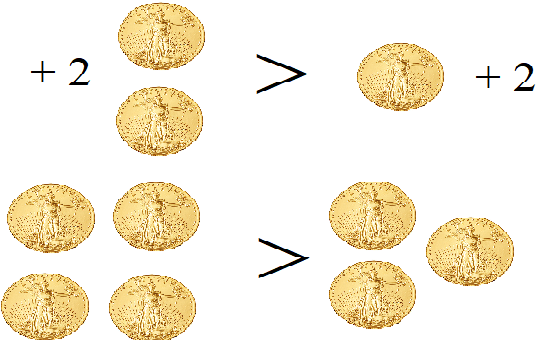
\includegraphics[scale=0.5]{Pictures/Coins.jpg}
\caption{Coins analogy}
\end{figure}

\noindent Extending onward with this analogy, if you have more coins in your right hand and you triple the number of coins in both hands, you will still have more coins in your right hand (multiplication). However, there will be instances where you will have to flip the direction of the inequality.

\pagebreak

\begin{center}
\noindent \underline{The following \textbf{will affect} the direction of the inequality:}
\begin{multicols}{2}
\begin{itemize}
    \item Multiplying or dividing by a \textbf{negative} number.
    \item Multiplying or dividing by a \textbf{variable}.
\end{itemize}
\columnbreak
\textbf{Example 3:}\\
$-10x > 40$\\
$x<-4$
\end{multicols}
\end{center}

%------------------------------------------------

\subsection{Multiplying and Dividing a Negative Number}\index{Multiply/Division by a Negative}
\begin{center}
\textbf{Whenever multiplying or dividing an inequality by a negative number, you must \emph{always} flip the inequality sign.}\\
\end{center}

\noindent Notice that we get a false statement when we multiply an inequality by -1 and do not flip the inequality sign.

\noindent\textbf{Example 4:}

\vspace*{-5mm}

\begin{center}
    $6>3$\\
    This is \textbf{True.}\\
    $\textbf{-1}*6>3*\textbf{-1}$\\
    $-6>-3$\\
    This is \textbf{false.}\\
\end{center}

\noindent The same thing will happen when dividing by a negative. The only way to prevent this is to flip the inequality sign to make this a true statement.
\begin{center}
    $-6<-3$\\
    This is \textbf{true.}\\
\end{center}
\noindent Due to this, it is always important to flip the inequality sign when multiplying or dividing by a negative number or else you will return a false statement.

%------------------------------------------------

\subsection{Multiplying and Dividing by an Unknown}

\begin{center}
    \textbf{You cannot multiply or divide by an unknown (such as a variable expression) unless you are sure of its sign.}\\
\end{center}

\noindent Since we will be working with rational inequalities, consider this inequality:

\noindent \textbf{Example 5:}

\begin{center}
    \LARGE{\textbf{$\frac{x+1}{x-6}\geq\frac{x+2}{x-4}$}}
\end{center}

\noindent You \textbf{cannot} cross multiply as you do not know whether the binomials are negative or not. Let's say you do cross multiply:

\begin{center}
\large{\textbf{$(x-4)(x+1)\geq(x+2)(x-6)$}}\\
\end{center}

\noindent If $(x-4)$ turned out to be negative (for example, if $x = -1$), it would turn out to be a false statement as you would be multiplying by a negative number and must flip the sign. Since we do not know whether the variable expressions in the inequality is positive or negative, we do not know whether to flip the sign or not. It is because of this we cannot cross multiply and will have to move all terms to one side, which will not cause a complication. We will learn how to solve rational inequalities in the next section.\\
\pagebreak

\noindent\textbf{Summary}:
\begin{itemize}
    \item You can solve inequalities by adding, subtracting, multiplying or dividing until you solve for the variable just like equations.
    \item You must flip the direction of the inequality sign when:
    \begin{itemize}
        \item Multiplying or dividing by a \textbf{negative} number.
    \end{itemize}
    \item Do not multiply or divide by an \textbf{unknown} unless you are sure of its sign. (if its always positive or always negative)
\end{itemize}
%------------------------------------------------
\vspace*{-6mm}
\section{Interval Notation}\index{Interval Notation}

\vspace*{-2mm}

\textbf{Interval Notation} is a way of representing subsets of the real number line. Interval notation will be commonly used for inequalities.\\

\vspace*{-3mm}

\noindent Interval notation uses a combination of square brackets "[ , ]" and parenthesis "( , )". For example, $(2,11]$ in interval notation, can be represented on a number line:

\noindent \textbf{Example 6:}

\begin{figure}[h]
\centering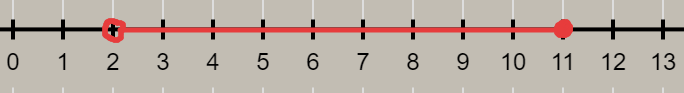
\includegraphics[scale=0.5]{Pictures/Example1.PNG}
\caption{\footnotesize{An open circle means we do not include that number, a closed circle means we do. $2<x\leq11$}}
\end{figure}

\vspace*{-3mm}

\noindent As you can see above, a bracket "[ , ]" means we include the endpoint while a parenthesis "( , )" means we do not. You can also use the infinity symbol to represent that the interval goes towards infinity. Note that infinities \textbf{never} gets a bracket, only parenthesis. It is not a number.

\noindent \textbf{Example 7:}

\vspace*{-12mm}

\begin{center}
    \large{$(-\infty,3]$:}
\end{center}

\vspace*{-8mm}

\begin{figure}[h]
\centering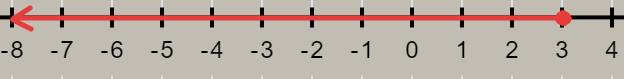
\includegraphics[scale=0.5]{Pictures/Example2.PNG}
\caption{\small{$x\leq3$ | Including 3 as it is a bracket.}}
\end{figure}

\vspace*{-8mm}

\begin{center}
\noindent \large{$(7,\infty)$:}
\end{center}

\vspace*{-15mm}

\noindent \textbf{Example 8:}

\begin{center}
\begin{figure}[h]
\centering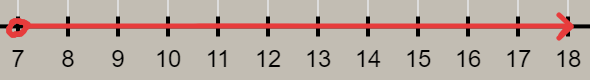
\includegraphics[scale=0.5]{Pictures/Example3.PNG}
\caption{\small{$x>7$ | Not including 7 as it is a parenthesis.}}
\end{figure}
\end{center}

\vspace*{-12mm}

\noindent When you have solved for the variable and have gotten a solution such as: $-3<x\leq6$, you will want to say: $x\in(-3,6]$. The $\in$ means "element of". A $\cup$ in between intervals means "union" or "or". A $\cap$ represents an intersection, or "and". There is another way of representing solutions called \textbf{Set Builder Notation}. We will quickly cover this as we will be using interval notation most of the time. $\{x\in\mathbb{R}|x>5\}$ reads: "x is a member of the set of real numbers such that x is greater than 5". 
\vspace*{-6mm}

%------------------------------------------------

\section{Exercises}\index{Exercises}

\small{To be more familiar with simple inequalities, attempt the following:}

\begin{exercise}
Solve and put in interval notation: $4(x+2)-1>5-7(4-x)$
\end{exercise}
\pagebreak
%------------------------------------------------

%----------------------------------------------------------------------------------------
%	CHAPTER 2
%----------------------------------------------------------------------------------------

\chapterimage{RationalGraphHeading.png}

\chapter{Rational Inequalities}

\vspace*{-18mm}

\noindent\normalsize Now that you have reviewed the basics on inequalities, let's move on to some more difficult ones. In this section, we will solve rational inequalities and explore related application problems. Rational functions can be applied in real life, such as finding out how fast two people can finish a job or how fast a river is flowing (rates). Since we will be focusing on inequalities, this section will assume you know the basics of Rational Functions. Solving rational inequalities is much like solving polynomial inequalities from last unit, as factoring and testing intervals are important concepts as well.

\vspace*{-6mm}

\section{Visualizing Rational Inequalities}\index{Visualizing Rational Inequalities}

It is good practice to visualize what we're actually doing instead of blindly solving without understanding what's happening. Let's consider:

\noindent\textbf{Example 9:}

\vspace*{-2mm}

\begin{center}
\begin{multicols}{2}
    \Large{$f(x) = \frac{(x+1)(x-3)^2}{(x-2)(x-5)^2}$}\\
\columnbreak
    \normalsize{Find when} \Large{$f(x) \leq 0$}
\end{multicols}
\end{center}

\vspace*{-3mm}

\begin{figure}[h]
\centering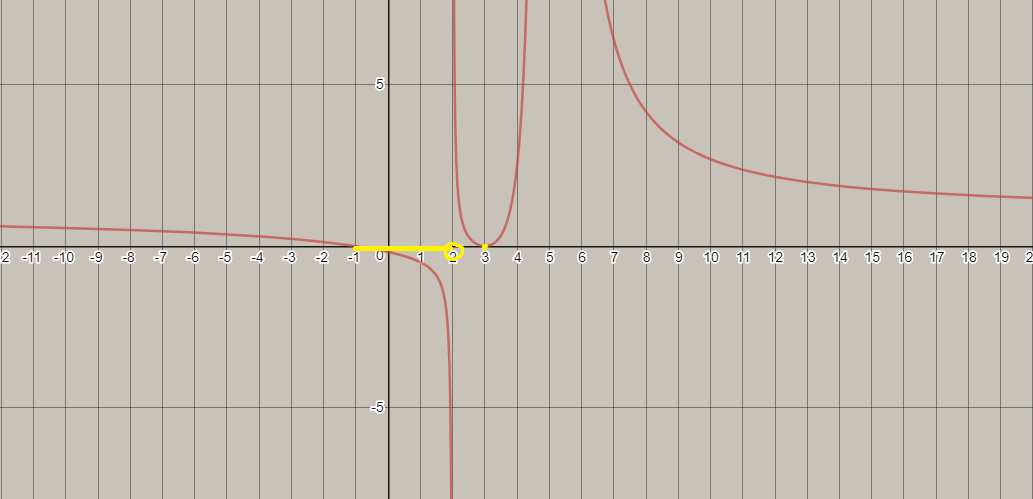
\includegraphics[scale=0.4]{Pictures/Graph1.png}
\caption{a graph of $f(x) = \frac{(x+1)(x-3)^2}{(x-2)(x-5)^2}$}
\end{figure}

\vspace*{-3mm}

\noindent Since we want to find when $f(x)$ is less than or equal to 0, we must look when the output or graph is on or below the x-axis, as the x-axis is at $f(x) = 0$. It is obvious that the graph crosses the x-axis at $x=-1$ and dips below the x-axis until the vertical asymptote at $x=2$. However, we do not include $x=2$ as it is a vertical asymptote and is undefined at that point. We must also include the x-intercept at $x=3$ as at that point, $f(x) = 0$. With all this information, we can say the solution is: $x\in[-1,2),\space x=3$.

%------------------------------------------------

\section{Solving Rational Inequalities}\index{Solving Rational Inequalities}

Solving rational inequalities is different than how we solve rational equations. Unlike with equations, we cannot cancel out the denominators by multiplying both sides by the least common denominator. You must first find the zeroes in the numerator and the undefined points in the denominator. You then use these points to divide the number line into intervals that you will then test for. The best way to learn is through some examples. 

\subsection{Simple Rational Inequalities}
Let's solve:

\noindent\textbf{Example 10:}

\begin{center}
    \LARGE{$\frac{3x+6}{2x-12}\leq0$}
\end{center}

\noindent Just like with polynomial inequalities, we want to get a zero on one side and a single rational on the other. We do not have to do this as it is already done. Next, we must factor the numerator and denominator as much as possible. We can pull out a 3 on the top and a 2 on the bottom. 

\begin{center}
    \LARGE{$\frac{3(x+2)}{2(x-6)}\leq0$}
\end{center}

\noindent Now solving for when the numerator and denominator equals 0, we can obviously see that $x=-2,6$ will be our key values. We use these numbers to test intervals as they are the only points where the function may change sign (positive to a negative, vice versa), similar to polynomial inequalities. There are two methods for testing intervals, you can plug in an x-value in each interval and check its sign or use a factor-table instead. I will be showing both methods.

\begin{center}
\textbf{Factor-Table}
\begin{table}[h]
\centering
\begin{tabular}{l l l l l l}
\toprule
\textbf{} & \textbf{$x<-2$\hspace{3mm}|} & \textbf{$x=-2$\hspace{5mm}|} & \textbf{$-2<x<6$\hspace{5mm}|} & \textbf{$x=6$\hspace{5mm}|} & \textbf{$x>6$}\\
\midrule
$x+2$ & \hspace{5mm}- & \hspace{5mm}0 & \hspace{12mm}+ & \hspace{3mm}+ & \hspace{5mm}+ \\
$x-6$ & \hspace{5mm}- & \hspace{5mm}- & \hspace{12mm}- & \hspace{3mm}0 & \hspace{5mm}+ \\
$\frac{3(x+2)}{2(x-6)}$ & \hspace{5mm}+ & \hspace{5mm}0 & \hspace{12mm}- & Undefined & \hspace{5mm}+ \\
\bottomrule
\end{tabular}
\end{table}
\end{center}

\vspace*{-4mm}

\noindent The factor-table has a row for each factor and one row for the whole function itself. Each row is split into columns with each representing one of the intervals on the number line and the key point itself. You must plug in values of x that satisfy the corresponding interval in each of the factors and place a + or - sign. For the last row, you simply figure out if the negatives cancel out or not and figure out the overall sign of the function. We are looking for when the function is less than or equal to zero. $\therefore -2\leq x<6$ or $x\in[-2,6)$

\pagebreak

\noindent The second method has you splitting up a number line based on the "key" values that you have found. We found two, so we will be splitting up our number line into three intervals.

\begin{figure}[h]
\centering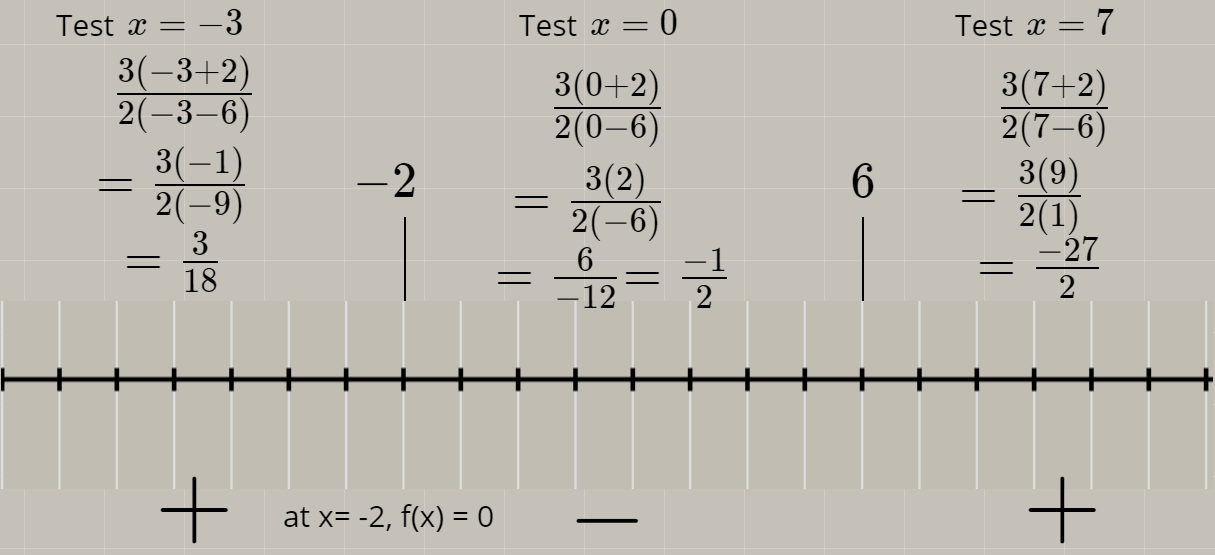
\includegraphics[scale=0.4]{Pictures/NumberLine1.PNG}
\caption{Number line method.}
\end{figure}

\noindent We tested whether the function was positive or negative at $x=-3,0,7$ by plugging in these values. The test at $x=-3$ had the negatives cancelling out, as can also be seen in the factor-table. Since we are looking for when the function is less than or equal to zero, we must include $x=-2$ as $f(x) = 0$ at that point, all the way to but not including $x=6$ as it is undefined there. $\therefore -2\leq x<6$ or $x\in[-2,6)$ The number line method could get long and is prone to errors, so using the factor-table is much more efficient. 

\subsection{Rational Inequalities w/ LCD}

Moving on to some more complicated problems, let's solve:

\noindent\textbf{Example 11:}

\vspace*{-5mm}

\begin{center}
    \LARGE{$\frac{x-8}{x} < \frac{3x+6}{2x+4}$}
\end{center}

\noindent The first thing we must do is move everything to one side to get a zero. As was explained before, we \emph{cannot} cross multiply for the reasons explained in section 1.3.2.

\vspace*{-4mm}

\begin{center}
    \LARGE{$\frac{x-8}{x} - \frac{3x+6}{2x+4} < 0$}
\end{center}

\noindent Let's factor to make the next step easier. We can factor out a 3 on the top and 2 on the bottom of the right most fraction. 

\vspace*{-4mm}

\begin{center}
    \LARGE{$\frac{x-8}{x} - \frac{3(x+2)}{2(x+2)} < 0$}
\end{center}

\noindent Next, we want to have a single rational expression on the left hand side to help identify our "key" values. We do this by combining the fractions, however, they must first have equal denominators. We will adjust the fractions based on the LCD. Remember to multiply by a fraction that is equal to one. (numerator and denominator are equal). This is also why the sign will \emph{not} flip here.

\vspace*{-4mm}

\begin{center}
    \LARGE{$\frac{(x-8)}{x} \cdot \frac{2(x+2)}{2(x+2)} - \frac{3(x+2)}{2(x+2)} \cdot \frac{x}{x} < 0$}
\end{center}

\begin{center}
    \LARGE{$\frac{2(x-8)(x+2)}{2x(x+2)} - \frac{3x(x+2)}{2x(x+2)} < 0$}
\end{center}

\pagebreak

\begin{center}
    \LARGE{$\frac{2(x-8)(x+2)-3x(x+2)}{2x(x+2)} < 0$}
\end{center}

\noindent Let's expand the numerator and simplify.

\begin{center}
    \LARGE{$\frac{2(x^2-6x-16)-(3x^2+6x)}{2x(x+2)} < 0$}
\end{center}

\begin{center}
    \LARGE{$\frac{2x^2-12x-32-3x^2-6x}{2x(x+2)} < 0$}
\end{center}

\begin{center}
    \LARGE{$\frac{-x^2-18x-32}{2x(x+2)} < 0$}
\end{center}

\begin{center}
    \LARGE{$\frac{-(x^2+18x+32)}{2x(x+2)} < 0$}
\end{center}

\noindent Now let's factor the numerator to identify our "key" values. Note: We can see we have a hole at $x=-2$ because the corresponding factors cancel. 

\begin{center}
    \LARGE{$\frac{-(x+16)(x+2)}{2x(x+2)} < 0$}
\end{center}

\noindent Now using what we learned, we can make this a bit easier for ourselves by multiplying both sides by -1. We learned when we do this, we must flip the inequality sign.

\begin{center}
    \LARGE{$\frac{(-(x+16)(x+2))(-1)}{2x(x+2)} < 0\cdot(-1)$}
\end{center}

\begin{center}
    \LARGE{$\frac{(x+16)(x+2)}{2x(x+2)} > 0$}
\end{center}

\noindent Now finding when the numerator and denominator equals 0, our "key" values are $x=-16,-2,0$. As stated before, there are two methods of testing intervals. Since the factor-table is more efficient, we will be using that method.

\begin{center}
\textbf{Factor-Table}
\begin{table}[h]
\begin{tabular}{l l l l l l l l}
\toprule
\textbf{} & \small{\textbf{$x<-16$}\hspace{3mm}|} & \small{\textbf{$x=-16$}\hspace{5mm}|} & \small{\textbf{$-16<x<-2$}\hspace{5mm}|} & \small{\textbf{$x=-2$}\hspace{5mm}|} & \small{\textbf{$-2<x<0$}}\hspace{5mm}| & \small{\textbf{$x=0$}}\hspace{5mm}| & \small{\textbf{$x>0$}}\\
\midrule
\small{$x+2$} & \hspace{5mm}- & \hspace{5mm}- & \hspace{12mm}- & \hspace{3mm}0 & \hspace{5mm}+ & \hspace{5mm}+ & \hspace{5mm}+\\
\small{$x+2$} & \hspace{5mm}- & \hspace{5mm}- & \hspace{12mm}- & \hspace{3mm}0 & \hspace{5mm}+ & \hspace{5mm}+ & \hspace{5mm}+\\
\small{$x+16$} & \hspace{5mm}- & \hspace{5mm}0 & \hspace{12mm}+ & \hspace{3mm}+ & \hspace{5mm}+ & \hspace{5mm}+ & \hspace{5mm}+ \\
\small{$x$} & \hspace{5mm}- & \hspace{5mm}- & \hspace{12mm}- & \hspace{3mm}- & \hspace{5mm}- & \hspace{5mm}0 & \hspace{5mm}+ \\
\small{$\frac{(x+2)(x+16)}{2x(x+2)}$} & \hspace{5mm}+ & \hspace{5mm}0 & \hspace{12mm}- & \small{Undefined} & \hspace{5mm}- & \small{Undefined} & \hspace{5mm}+ \\
\bottomrule
\end{tabular}
\end{table}
\end{center}

\noindent To better understand how to quickly get the signs for the last row, here is what's happening. We know $(x+2)$, $(x+16)$, and $x$ is negative. So let's just substitute it for its respective signs. Another method is using bounce's, cut's and bend's to determine signs, however, you must be very comfortable with graphing rational functions.

\pagebreak

\begin{center}
\begin{multicols}{2}
\LARGE{$\frac{(x+16)(x+2)}{2x(x+2)}$}\\
\columnbreak
\LARGE{$\frac{(-)(-)}{(-)(-)}> 0$}\\
\end{multicols}
\end{center}

\noindent Here, you can clearly see the negatives cancel out. Repeat for the rest of the table.

\noindent Since we want when the function is positive (and not equal to zero), we can see the positive intervals are at $x<-16$ and $x>0$. $\therefore x\in (-\infty,-16)\cup(0,\infty)$ Using desmos, we can verify our answer. $\frac{x-8}{x}$ is the red graph and $x\in (-\infty,-16)\cup(0,\infty)$ is when it is less than the green graph which is $\frac{3x+6}{2x+4}$.\\

\vspace*{-12mm}

\begin{center}
    \large{\textbf{Original:}}\\
    \LARGE{$\frac{x-8}{x}<\frac{3x+6}{2x+4}$}\\
\end{center}

\vspace*{-5mm}

\begin{figure}[h]
\centering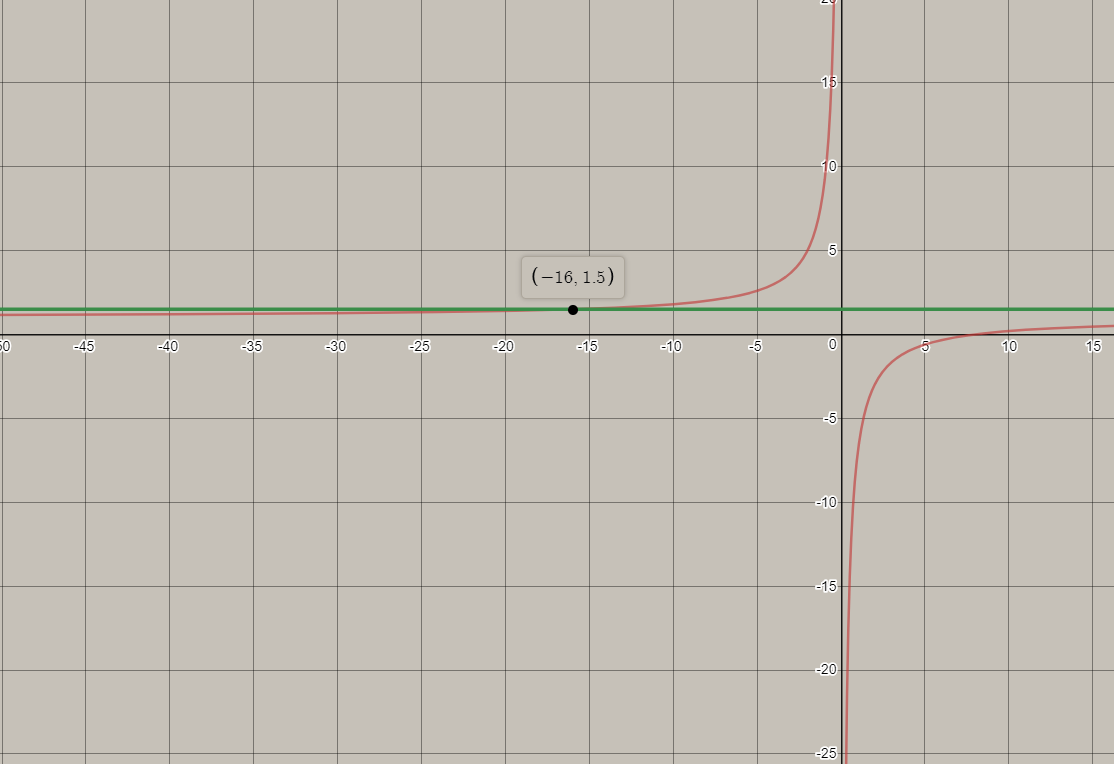
\includegraphics[scale=0.3]{Pictures/Proof1.PNG}
\caption{a graph of $\frac{x-8}{x}$ and $\frac{3x+6}{2x+4}$}
\end{figure}

\noindent As you can see, the green graph ($\frac{3x+6}{2x+4}$), is looking like a horizontal line. This is because when you factor it to $\frac{3(x+2)}{2(x+2)}$, the $(x+2)$ cancels out completely. \\

\vspace*{-6mm}

\begin{center}
    \LARGE{$f(x)=\frac{3(x+2)}{2(x+2)}$}\\
    \LARGE{$f(x)=\frac{3}{2}$}\\
\end{center}

\noindent However, with rationals, you should remember that when factors cancel out, there is a hole at that corresponding x-value. For example, a cancelled out $(x+2)$ factor means there is a hole at $x=-2$. Since it ends up being just $f(x)=\frac{3}{2}$, it makes sense that it is a horizontal line at $y=1.5$.\\

\noindent We can check our answer algebraically as well. We can just plug in a point that is in our interval answer and check if it does satisfy the inequality. 

\begin{center}
    \textbf{Test $x=8$}\\
    \large{$\frac{x-8}{x} < \frac{3x+6}{2x+4}$}\\
    \vspace{2mm}
    \large{$\frac{8-8}{8} < \frac{3(8)+6}{2(8)+4}$}\\
    \vspace{2mm}
    \large{$\frac{0}{8} < \frac{30}{20}$}\\
    \vspace{1mm}
    \large{$0 < \frac{3}{2}$}\\
\end{center}

\noindent It is possible to solve this without moving all the terms to one side. You just need to identify all the "key" values and plug in the values in the whole inequality and checking if it satisfies it. For example, plugging in $x=-3$ in $\frac{x-8}{x} < \frac{3x+6}{2x+4}$. Much like we do when solving irrational inequalities.

%------------------------------------------------

\section{Applications}\index{Applications}

Applications in real life include finding when an average cost function, $\frac{80x+150}{x}$ is less than 100. Meaning, how much items you need to produce so that the average cost is less than 100. 

%------------------------------------------------

\section{Exercises}\index{Exercises}

To be more familiar with rational inequalities, try the following:

\begin{exercise}
Solve: $\frac{x-8}{x}\leq3-x$
\end{exercise}

%----------------------------------------------------------------------------------------
%	CHAPTER 3
%----------------------------------------------------------------------------------------

\chapterimage{Pictures/IrrationalHeading.PNG} % Chapter heading image

\chapter{Irrational Inequalities}

\noindent Solving irrational inequalities, much like rational inequalities, include testing intervals as well. The only difference is that we must first figure out the domain, and solve the related equation as squaring both sides of an inequality will need a flip (in certain cases). 

\section{Squaring Both Sides of an Inequality}

\noindent We can only square both sides of an inequality if we know that both sides are positive. Consider this:\\
\textbf{Example 12:}

\vspace*{-5mm}

\begin{center}
    $5<6$\\
    $5^2<6^2$\\
    $25<36$\\
    \textbf{True}\\
\end{center}


\noindent When we square both sides that are positive, you can see the inequality still holds true. 

\noindent\textbf{Example 13:}

\vspace*{-5mm}

\begin{center}
    $-5>-6$\\
    $(-5)^2>(-6)^2$\\
    $25>36$\\
    \textbf{False}\\
\end{center}

\vspace*{-3mm}

\noindent However, when we square both sides that are negative, you can see the inequality becomes false. If we do not know whether both sides are positive or negative, we cannot square both sides of an inequality.

\pagebreak

\section{Solving Irrational Inequalities}\index{Solving Irrational Inequalities}

\noindent Let's try solving:

\noindent\textbf{Example 14:}

\begin{center}
    \LARGE{$\sqrt{x^2-4x}<6-x$}
\end{center}

\noindent First, we must figure out the domain. We can do this by simply solving when $x^2-4x\geq0$ as the radicand (terms under the square root) cannot be negative. This ties into review from polynomial inequalities. 

\vspace*{-4mm}

\begin{figure}[h]
\begin{center}
\textbf{Domain:}\\
    $x^2-4x\geq0$\\
    $x(x-4)\geq0$\\
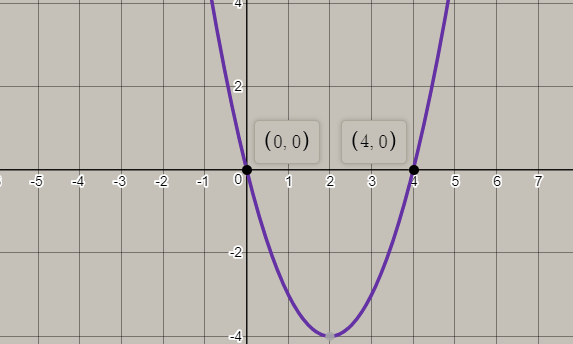
\includegraphics[scale=0.75]{Pictures/Graph2.PNG}
\caption{a graph of $x^2-4x$}
\end{center}
\end{figure}

\vspace*{-7mm}

\noindent For a review of polynomial inequalities, you want to factor the polynomial so you can see the roots. From there, you want to see if the parabola is opening upward or downward and sketch appropriately. You can then see at what intervals the graph is above or below zero. From the figure above, it is obvious the graph is greater than or equal to 0 at the intervals: $(-\infty,0]\cup[4,\infty)$.\\

\noindent Since we know the domain is: $x\in(-\infty,0]\cup[4,\infty)$. We need to solve the related equation next. The related equation will just switch out the inequality sign for an equal sign. From there we can square both sides as it is no longer an inequality.

\begin{center}
    \textbf{Related Equation:}\\
    \Large{$\sqrt{x^2-4x}=6-x$}\\
    \Large{$(\sqrt{x^2-4x})^2=(6-x)^2$}\\
    \Large{$x^2-4x=(6-x)(6-x)$}\\
    \Large{$x^2-4x=36-6x-6x+x^2$}\\
    \Large{$x^2-4x=x^2-12x+36$}\\
    \Large{$8x=36$}\\
    \Large{$x=\frac{36}{8}$}\\
    \Large{$x=\frac{9}{2}$}\\
\end{center}

\noindent We have just found out that at $x=\frac{9}{2}$, both graphs, $\sqrt{x^2-4x}$ and $6-x$, are equal (POI). Now just like with the previous inequalities, we must test intervals. We can split up the number line into 4 intervals using the domain and the solution of the related equation and test. We then plug in values in the corresponding intervals and check which is true or false. 

\begin{center}
\textbf{Factor-Table}
\begin{table}[h]
\centering
\begin{tabular}{l l l l l l}
\toprule
\textbf{} & \textbf{$x<0$\hspace{3mm}|} & \textbf{$0<x<4$\hspace{5mm}|} & \textbf{$4< x<\frac{9}{2}$\hspace{5mm}|} & \textbf{$\frac{9}{2}<x$}\\
\midrule
{$\sqrt{x^2-4x}<6-x$} & \hspace{5mm}True & \hspace{5mm}Error & \hspace{5mm}True & \hspace{3mm}False &\\
\bottomrule
\end{tabular}
\end{table}
\end{center}

\begin{multicols}{2}
\begin{center}
    \textbf{x=-1}\\
    $\sqrt{(-1)^2-4(-1)}<6-(-1)$\\
    $\sqrt{1+4}<7$\\
    $\sqrt{5}<7$\\
    $\approxeq2.236<7$\\
    \textbf{True}\\
    \columnbreak
    \textbf{x=2}\\
    $\sqrt{(2)^2-4(2)}<6-(2)$\\
    $\sqrt{4-8}<4$\\
    $\sqrt{-4}<4$\\
    \textbf{Error}\\
\end{center}
\end{multicols}

\begin{multicols}{2}
\begin{center}
    \textbf{x=4.2}\\
    $\sqrt{(4.2)^2-4(4.2)}<6-(4.2)$\\
    $\sqrt{17.65-16.8}<1.8$\\
    $\sqrt{0.85}<1.8$\\
    $\approxeq0.921<1.8$\\
    \textbf{True}\\
    \columnbreak
    \textbf{x=6}\\
    $\sqrt{(6)^2-4(6)}<6-(6)$\\
    $\sqrt{36-24}<0$\\
    $\sqrt{12}<0$\\
    $\approxeq3.464<0$\\
    \textbf{False}\\
\end{center}
\end{multicols}

\begin{multicols}{3}
\begin{center}
    \textbf{x=0}\\
    $\sqrt{(0)^2-4(0)}<6-(0)$\\
    $\sqrt{0}<6$\\
    $0<6$\\
    \textbf{True}\\
    \columnbreak
    \textbf{x=$\frac{9}{2}$}\\
    $\sqrt{(\frac{9}{2})^2-4(\frac{9}{2})}<6-(\frac{9}{2})$\\
    $\sqrt{\frac{81}{4}-\frac{36}{2}}<\frac{12}{2}-\frac{9}{2}$\\
    $\sqrt{\frac{81}{4}-\frac{72}{4}}<\frac{3}{2}$\\
    $\sqrt{\frac{9}{4}}<\frac{3}{2}$\\
    $\frac{3}{2}<\frac{3}{2}$\\
    \textbf{False}\\
    \columnbreak
    \textbf{x=4}\\
    $\sqrt{(4)^2-4(4)}<6-(4)$\\
    $\sqrt{16-16}<2$\\
    $\sqrt{0}<2$\\
    $0<2$\\
    \textbf{True}\\
\end{center}
\end{multicols}

\noindent All we need to do is include everything that satisfies the inequality in interval notation. We can test the endpoints of the intervals as well. Our answer comes out to be: $x\in(-\infty,0]\cup[4,\frac{9}{2})$.\\

\pagebreak

\noindent Using desmos we can quickly verify our answer. $\sqrt{x^2-4x}$ is the purple graph and $6-x$ is the green graph.

\begin{figure}[h]
\centering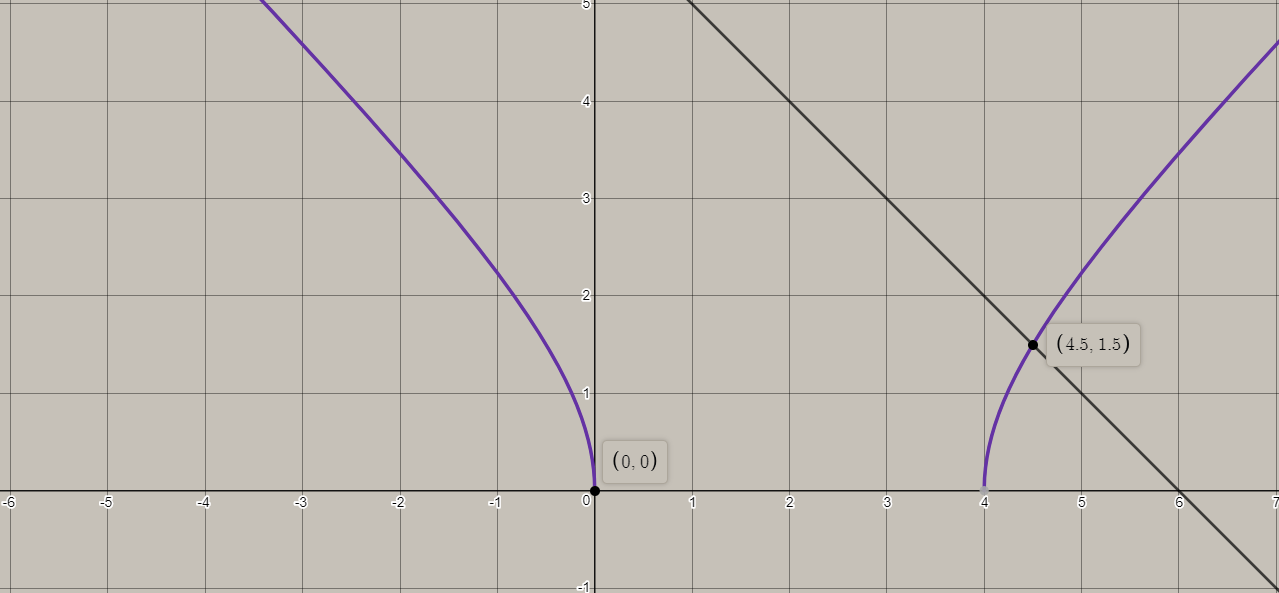
\includegraphics[scale=0.4]{Pictures/Graph3.PNG}
\caption{a graph of $\sqrt{x^2-4x}$ and $6-x$}
\end{figure}

\noindent As a summary, solving rational inequalities are much like regular equations, but you have to keep in mind all the rules taught in the first section. You must fully factor the rational expressions to successfully identify the "key" values. You then use these "key" values to split the number line into intervals to test for. There are two methods, the factor-table and number line method. The factor-table is much more efficient and less prone to errors. Solving irrational inequalities include solving for the domain and then the related equation. This is because there are exceptions when squaring both sides of an inequality. You then use these "key" values to split the number line and plug into the original inequality. Applications of rational inequalities in real life include solving for when the average cost of a product will be less than 100.  In the Calculus and Vectors course we can find out the turning points of the graph by finding the derivative of the function and setting it to zero. 


\section{ANSWER KEY}\index{Answer Key}

\Large{\textbf{Exercise 1.1}}\\
\large{\textbf{Answer}: $x<10$ \hspace{5mm} | \hspace{5mm} $x\in(-\infty,10)$}\\

\vspace{4mm}

\noindent\Large{\textbf{Exercise 2.1}}\\
\large{\textbf{Answer}: $x\leq-2$ or $0<x\leq4$ \hspace{5mm} | \hspace{5mm} $x\in(-\infty,-2]\cup(0,4]$}\\

%----------------------------------------------------------------------------------------
%	INDEX
%----------------------------------------------------------------------------------------

\cleardoublepage % Make sure the index starts on an odd (right side) page
\phantomsection
\setlength{\columnsep}{0.75cm} % Space between the 2 columns of the index
\addcontentsline{toc}{chapter}{\textcolor{ocre}{Index}} % Add an Index heading to the table of contents
\printindex % Output the index

%----------------------------------------------------------------------------------------

\end{document}
